\documentclass[12pt]{report}

\usepackage{amssymb,amsthm}
\usepackage{amsmath,color}
%\usepackage{dsfont}
\usepackage{setspace}
\usepackage{graphicx}
\usepackage{multicol}
\usepackage[document]{ragged2e}


\def\w{\mathtt w}
\def\K{\mathcal K}
\def\N{\mathbb N}
\def\R{\mathcal R}
\def\l{\ell}
\def\S{\mathcal S}
\def\Z{\mathbb Z}
\def\ora{\overrightarrow}

\newtheorem{theorem}{Theorem}[section]
\newtheorem{corollary}{Corollary}[theorem]
\newtheorem{lemma}[theorem]{Lemma}
\begin{document}

\begin{center}
\LARGE{\textbf{Indian Institute of Technology, Delhi}}\\
\vspace{1cm}
\large{\textbf{Design Practices in Computer Science}}\\[5pt]
\large{\textbf{COP290}}\\[5pt]
\large{\textbf{Mathematical Model}}\\[5pt]
%by \\
\vspace{0.5cm}

\large{\textbf{Design and Implement a Software }}
\large{\textbf{\\for Engineering Drawing}}\\[5pt]



%\vspace{1in}

\begin{center}
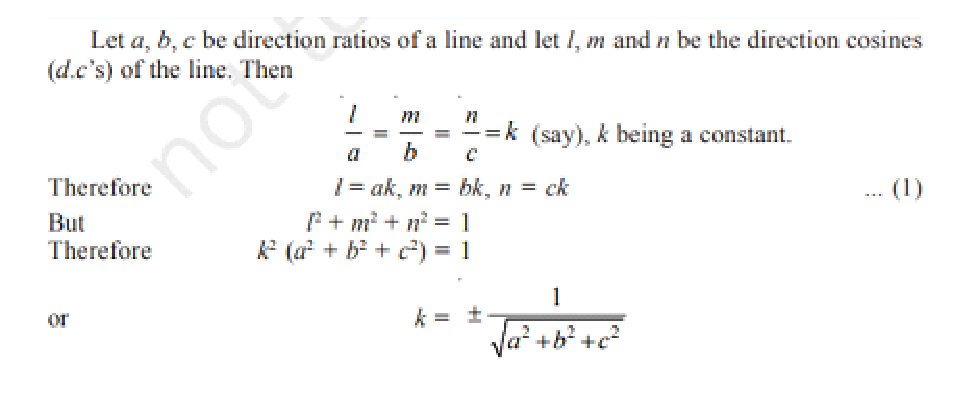
\includegraphics[height=4.5cm]{image5.eps}
\end{center}
\vspace{0.2cm}

\textbf{January 18, 2018} \\
\textbf{Department of Computer Science and Engineering} \\
%\textbf{Indian Institute of Technology, Delhi}\\
%\textbf{16 January 2018}


\vspace{2cm}


\begin{multicols*}{2}

\begin{flushleft}

\textit{Authors :\\ }


\textbf{Udit Jain} \\
(2016CS10327)\\
\textbf{Shashank Goel}
(2016CS10332)\\

\end{flushleft}


\columnbreak

\begin{flushleft}

\textit{\\Supervisor :\\ }
\textbf{Prof. Subhashish Bannerjee} \\[5pt]

\end{flushleft}

\end{multicols*}

\end{center}

\newpage



\begin{center}
\Large \bf ABSTRACT
\end{center}
\vspace{0.2in}

We are going to design and implement a Software Package for Engineering drawing that shall be described and portrayed in a series of five steps to finely work out the design, analysis and the modelling.
\\
\vspace{0.3cm}
The package will have the following functionalities:

\begin{enumerate}
  \item
  We will be able to interactively input or read from a file either
  \begin{itemize}
    \item
    An isometric drawing and a 3D object model 
    \item
    Projections onto any cross section
  \end{itemize}
  \item
  For a given 3D model description, the software will be able to \textit{generate projections} onto any cutting plane or any cross section
  \item
  Given two or more projections, we will be able to interactively \textit{reconstruct the 3D model} of the object and produce the isometric view along any view direction

\end{enumerate}

\vspace{0.5cm}
In this design project, we shall work as developers and algorithm enthusiasts to understand the ways and finding different means to approach and tackle the objectives in a more well defined mathematical way. The solutions shall be presented not completely on how the human brain formulates or understands/interprets a given figure, be it 2D or 3D but in a way, that shall work out in all the cases we deal with in real life and definitely be understandable by the machine. Mathematical explanations that are more amenable to intuition are given.

\vspace{0.2cm}

Being an amateur in this field of design of software to compute projections and reconstruction of the model, it might eventually happen that the algorithm might fail in some cases or it may be proved that such an algorithm cannot exist or the model be correct but be based on certain assumptions on the construction of the object or the projections. Nevertheless, we shall work with full confidence and zeal to achieve the goal or reach to quite an end of the problem so that using our lemmas, proofs and knowledge, someday a perfect model can be implemented using a software by some other Computer Explorer. 
\\
\vspace{0.2cm}

As a matter of interest, we just wish to argue that these things can be computed by our brain so we do hope to find a solution to this problem using machine learning algorithms. Since, Machine Learning algorithms are more or less based on Mathematical matrices, with the use of computer graphics, we expect to find a start with matrices that we have dealt with further in this report. 

\newpage

\tableofcontents

\newpage

\chapter{Introduction}

In the last ten years, a significant progress occurred in the area of 3D graphics. Many studies have been conducted in the field of 3D modeling, and a variety of methods that allow us to reconstruct 2D images into 3D were created. Today, 3D graphics industry creates models that can no longer be distinguished from a person in the real world or on photograph. This way of modeling is also the goal of this work; to explore options to create a photo-realistic 3D model shaped from the 2D images. This article has listed and briefly described methods of converting 2D images into 3D models.
\vspace{1cm}

The following objectives are aimed to be covered in this paper:

\begin{itemize}
  \item
  Working out a mathematical description of the problem.
  \item
  Figure out how many views are necessary for reconstruction.
  \item
  Figure out how many views are sufficient for reconstruction.
  \item
  How to compute the projections from the 3D model?
  \item
  How to produce the isometric view using one or more projections?
  \item
  What interactions are necessary?
  
\end{itemize}

\vspace{0.5cm}

We shall study the direction cosines and direction ratios of a line joining two points and also discuss about the equations of lines and planes in space under different conditions, angle between two lines, two planes, a line and a plane, shortest distance between two skew lines and distance of a point from a plane. Most of the above results are obtained in vector form. Nevertheless, we shall also translate these results in the Cartesian form which, at times, presents a clearer geometric and analytic picture of the situation.
\\
\vspace{0.5cm}

We shall further study the Vector Algebra and the 3D Transformations required to convert a given 3D Object to its projection view on any cross section and also do the same in a reverse manner i.e. converting the given projections back into the 3D Object by using matrices and their properties trying to exploit as many as possible and making them use to determine the number of different possible reconstructions possible (if any). We shall describe the assumptions while formulating the problem and prove to detail all the lemmas and theorems that are being used to define the model.
\\

\chapter{Vector Algebra and 3D Transformation}

\section{Homogeneous coordinate System}

Three-dimensional scene description requires mainly using a 3D Cartesian coordinate system. Points in space are uniquely determined by their three \textit{ Cartesian coordinates $(x, y, z)$ } .

\vspace{0.5cm}
\noindent Of greater importance for computer graphics is the usage of \textit{ homogeneous} or \textit{projective coordinates }. Ordinary points in space are given four coordinates instead of three:


\subsection{Introduction}

\begin{center} 
\[ ( x , y , z ) \Leftrightarrow ( x , y , z , w ) \]
\end{center}

\vspace{.3cm}
This coordinate system has wide range of applications, including computer graphics and 3D computer vision, where they allow affine transformations and projective transformations to be easily represented by a matrix
\\
\vspace{.3cm}

This introduces an obvious redundancy, so that the same point in 3D has infinitely many homogeneous coordinates, according to the equivalence
\\
\vspace{.3cm}

\begin{center} 
\[ (x, y, z, w) \equiv (x_{0}, y_{0}, z_{0}, w_{0})   \Leftrightarrow \alpha \hspace{0.2cm} (x, y, z, w) =  (x_{0}, y_{0}, z_{0}, w_{0})  \]
\end{center}


\subsection{Homogeneous Matrix}

\noindent The concatenation of a translation with a rotation, scaling or shear requires an awkward combination of a matrix addition and a matrix multiplication. The problem can be avoided by using an alternative coordinate system for which computations are performed by 3 × 3 matrix multiplications. Since 

\begin{center}
\[ (x' \hspace{.2cm}  y' \hspace{.2cm}  l ) \hspace{.2cm} = \hspace{.2cm} (x' \hspace{.2cm}  y' \hspace{.2cm} l )    \hspace{0.2cm} \begin{pmatrix}
a & d & 0 \\
b & e & 0 \\
c & f & 1 
\end{pmatrix} \]
  
\end{center}

To this end a new coordinate system is defined in which the point with Cartesian coordinates $ (x , y) $ is represented by the homogeneous or projective coordinates $( x , y , 1 )$, or any multiple $( rx , ry , r )$ with $ r \neq 0 $.


\vspace{.5cm}
The set of all homogeneous coordinates $(x , y , w)$ is called the \textit{projective plane} and denoted $ P^2 $. In order to carry out transformations using matrix computations the homogeneous coordinates $( x, y, w )$ are represented by the row matrix $(x, y, w)$. 

\vspace{.5cm}

\hspace{1cm} The above equation implies that any planar transformation can be performed by a $ 3 × 3 $ matrix multiplication and using homogeneous coordinates. Sometimes homogeneous coordinates will be denoted by capitals $ (X, Y, W) $  in order to distinguish them from the affine coordinates $(x, y)$.


\subsection{Key Aspects}
\begin{itemize}
  \item 
  Any point in the projective plane is represented by a triple $ (X,Y,Z) $ , called the\textit{ homogeneous coordinates } or\textit{ projective coordinates }of the point, where$ X Y $ and$ Z $ are not all $ 0 $ .
  \item 
  The point represented by a given set of homogeneous coordinates is unchanged if \textit{  the coordinates are multiplied by a common factor }.
  \item 
  Conversely, two sets of homogeneous coordinates represent the same point if and only if one is obtained from the other by multiplying all the coordinates by the same  \textit{ non-zero constant }.
  \item 
  When$ Z $ is not $ 0$  the point represented is the point$ (X/Z,Y/Z)$ in the Euclidean plane.
  \item 
  When$ Z $ is $ 0$  the point represented is a point at $ infinity $ .
\end{itemize}

\section{Vector Algebra}


\hspace{1cm} In mathematics and linear algebra,vector algebra refers to algebraic operations in vector spaces. Most commonly, it refers to operations on Euclidean vectors.

\subsection{Vector Operations}

Vectors in 3D space are usually given by their Cartesian coordinates, and operations on vector can be defined in terms of them:

\indent \textbf{\textit{Addition : }} $ (x, y, z) + (x’ , y’ ,z’) = (x + x’, y + y’, z + z’) $  \\
\indent \textbf{\textit{Subtraction : }} $(x, y, z) − (x’ , y’ ,z’) = (x – x’ ,y – y’, z – z’)$ \\
\indent \textbf{\textit{Scaling : }} $ \lambda (x, y, z) = (\lambda x, \lambda y, \lambda z)  $ \\
\indent \textbf{\textit{Dot Product : }}$ (x, y, z) \cdot (x_{0} , y_{0} ,z_{0} ) = x x_{0} + y y_{0} + z z_{0} $ \\
\indent \textbf{\textit{Norm : }} $ \| ( x , y , z ) \| = \sqrt{\vert \overrightarrow{v} \cdot \overrightarrow{v} \vert } = \sqrt{x^2 + y^2 + z^2} $ \\
\indent \textbf{\textit{Cross Product : }} $ (x, y, z ) \times (x_{0} , y_{0} ,z_{0} ) = (y z_{0} − z y_{0} ,z x_{0} − x z_{0} , x y_{0} − y x_{0} ) $ \\

\subsection{Geometric Interpretation}

The dot product is fundamentally a projection. The dot product of a vector with a unit vector is the projection of that vector in the direction given by the unit vector. This is given by the formula:

\[ \overrightarrow{v} \cdot \overrightarrow{w} = \vert \overrightarrow{v} \vert \vert \overrightarrow{w} \vert  cos (\theta) \]


Furthermore, it follows immediately from the geometric definition that two vectors are orthogonal if and only if their dot product vanishes, that is : 

\[ \overrightarrow{v} \bot \overrightarrow{w} \Leftrightarrow \overrightarrow{v} \cdot \overrightarrow{w} = 0 \]


The component form of the dot product now follows from its properties given above. For example, 

\[ \overrightarrow{v} \cdot \overrightarrow{w} = ( v_{x} \widehat{i} + v_{y} \widehat{j}) \cdot ( w_{x} \widehat{i} + w_{y} \widehat{j}) = v_{x}w_{x} + v_{y}w_{y} \] 

\indent \textbf{Orthogonal : } Two vectors are orthogonal if their dot product is zero.  
\indent \textbf{Collinear : } Two vector are collinear if their cross product is zero.  
\indent \textbf{Normal : } A normal vector to the plane defined by $\overrightarrow{v}  $ and $ \overrightarrow{w}$ is given by  $\overrightarrow{v} \times \overrightarrow{w}  $

\subsection{Direction Cosines}

$
If a directed line \mathcal{L} passing through the origin makes angles \alpha, \beta and \gamma with x, y and z-axes, respectively, called direction angles, then cosine of these angles, namely, cos \alpha, cos \beta and cos \gamma are called direction cosines of the directed line \mathcal{L} . If we reverse the direction of L, then the direction angles are replaced by their supplements, i.e., \pi - \alpha , \pi - \beta and \pi - \gamma . Thus, the signs of the direction cosines are reversed. 
$
\vspace{0.3cm}
Note that a given line in space can be extended in two opposite directions and so it has two sets of direction cosines. In order to have a unique set of direction cosines for a given line in space, we must take the given line as a directed line. These unique direction cosines are denoted by l, m and n. \\
\vspace{0.5cm}

Let a,b,c be the direction ratios of a line and let l , m and n be the direction cosines \textit{(d.c's)} of the line. Then,

\[ \dfrac{l}{a} = \dfrac{m}{b} = \dfrac{n}{c} = k (constant) \]
Therefore \[ l = ak, m = bk , n = ck \]
But       \[ l^2 + m^2 + n^2 = 1 \]
Therefore \[ k^2 (a^2 + b^2 + c^2) = 1 \]

\[ k = \pm \dfrac{1}{ \sqrt{a^2 + b^2 + c^2} } \]

\section{Transformations on 3D Objects}

$
A\textbf{transformation}is a function f that maps a set \chi to itself, i.e.f:\chi \rightarrow \chi. Examples include rotations, reflections and translations. These can be carried out in Euclidean space, particularly in\mathbb{R}^2and\mathbb{R}^3. They are also operations that can be described explicitly using matrices.
$

\subsection{Translation}
Translation is one of the most basic operations that can be performed on an object. It can be defined as the elementary transformation which can preserve relative positions of any two points in the coordinate space. 
\vspace{0.3cm}
\\
A translation is a transformation which maps a point P (x, y) to a point $ P' (x’ , y’) $by adding a constant amount to each coordinate so that 
\[ x' = x + h, y' = y + k \] for some constants h and k.

\[ R_{x}(\theta) = \begin{bmatrix}
1 & 0 & 0 \\
0 & cos(\theta) & -sin(\theta) \\
0 & sin(\theta) & cos(\theta) 
\end{bmatrix} \]


\[ R_{y}(\theta) = \begin{bmatrix}
cos(\theta) & 0 & sin(\theta) \\
0 & 1 & 0 \\
-sin(\theta) & 0 & cos(\theta) 
\end{bmatrix} \]


\[ R_{z}(\theta) = \begin{bmatrix}
cos(\theta) & -sin(\theta) & 0 \\
sin(\theta) & cos(\theta) & 0 \\
0 & 0 & 1 
\end{bmatrix} \]

In general, for the case of the 3D coordinate system the translation is defined by the following rules:

\[ 		x’ = x + h	y’ = y + k	z’ = z + l  \]

\subsection{Rotation}

A rotation about the origin through an angle $ \theta$ has the effect that a point P(x, y) is mapped to a point $ P’ (x’ , y’) $ so that the initial point P and its image point $ P' $ are the same distance from the origin, and the angle between lines OP and $ OP’ $ is $ \theta $ .
\vspace{0.3cm}

\hspace{1cm} Since we have been considering the fact that matrices are important in the study of coordinate geometry involving projections, we must not proceed without getting the glimpse of this transformation in terms of matrices. The Rotation of the coordinate system about the conventional orthogonal axis of rotation and along any axis is specified below.
\vspace{0.3cm}
It might be quite intriguing to the reader how the rotation of a point about a given axis can actually be synced or thought about to be multiplication with a matrix. 

\begin{lemma}
  Multiplication of a matrix, having a unit determinant and transpose same as its inverse, with any point vector in the coordinate space essentially amounts to its rotation around a fixed axis and by a fixed angle.
\end{lemma}

\begin{enumerate}
  \item Anti-clockwise Rotation about x-axis by an angle$ \theta$.
  \item Anti-clockwise Rotation about y-axis by an angle$ \theta$. 
  \item Anti-clockwise Rotation about z-axis by an angle$ \theta$. 
\end{enumerate}

\subsection{General Rotation about any Axis}

$
In order to get the rotation matrix for rotation about any axis with direction cosines u_{x}, u_{y},u_{z} by an angle \theta is given by : 
$
\[ R =  \begin{bmatrix}
cos(\theta) + u_{x}^2(1-cos(\theta)) & u_{x}u_{y}(1-cos(\theta)) - u_{z}sin(\theta) &  u_{x}u_{z}(1-cos(\theta)) + u_{y}sin(\theta) \\
u_{y}u_{z}(1-cos(\theta)) + u_{z}sin(\theta) & cos(\theta) + u_{y}^2(1-cos(\theta)) &  u_{y}u_{z}(1-cos(\theta)) - u_{x}sin(\theta) \\
u_{z}u_{x}(1-cos(\theta)) - u_{y}sin(\theta) & u_{z}u_{y}(1-cos(\theta)) + u_{x}sin(\theta) & cos(\theta) + u_{z}^2(1-cos(\theta)) 
\end{bmatrix}\]

\subsection{A simple derivation for the case of 2D view}

First of all, it must been seen that rotating about any of the orthogonal axis is , in practice a rotation in the traditional 2D plane. This is because one of the parameter of the position triple has to be the same after rotation depending upon which axis you choose to rotate about. Thus the general two dimensional matrix can be easily extended to simple three dimensional case.
\vspace{0.3cm}
\\The rotation about the origin in the x-y pplane corresponds to the following matrix that we wish to derive:
\[ \begin{bmatrix}
cos(\theta)  &  -sin(\theta) \\
sin(\theta)  &  cos(\theta) \\
\end{bmatrix}\]

\hspace{1cm} The derivation of the new coordinates of a generic point P can be inferred from the geometry that has been presented in the following figure:
\\
\vspace{0.2cm}

The matrix
\[ S(s_{x},s_{y}) = \begin{pmatrix}
s_{x} & 0 \\
0 & s_{y}
\end{pmatrix}  \]
\begin{center}
  is called the \textit{scaling transformation matrix.}

  An Image will come Here(cropped?)
  \vspace{4cm}
\end{center}

The coordinates$ (x’ , y’ ) $can be obtained from$ (x, y) $by the matrix multiplication

\[ \textbf{P} = (x \hspace{0.3cm} y) \begin{pmatrix}
cos(\theta) & sin(\theta) \\
-sin(\theta) & cos(\theta)
\end{pmatrix} = (x cos(\theta) - y sin(\theta) \hspace{0.3cm} x sin(\theta) + y cos(\theta) ) \]

The matrix:

\[ Rot(\theta) = \begin{pmatrix}
cos(\theta) & sin(\theta) \\
-sin(\theta) & cos(\theta)
\end{pmatrix} \]

is called the \textit{Rotation Matrix}.\\


The reader must notice that the rotation matrices may have a difference in sign of θ. Because of the direction of rotation that we might decide.\\

\subsection{Scaling}

Scaling is a linear transformation that enlarges or shrinks an object by scale factors that may or may not be equal in all directions. The scaling matrix is any diagonal matrix with positive reals as elements.\\
\vspace{0.3cm}

A scaling about the origin is a transformation which maps a point$ P(x, y) $to a point$ P’ (x’ , y’ ) $by multiplying the x and y coordinates by non-zero constant scaling factors sx and sy, respectively, to give $ x’ = S_{x} X and y’ = S_{y} Y$ .
\vspace{0.3cm}
\\
Scaling is not as such a very useful tool to change the view angle or just change the position of the object but enables us to change its size (as seen by us) with a given viewing screen or better say field of view.

\section{Tools for Projection/Reconstruction}

The powerful theory described above will be used to prove more results that we will see in the upcoming chapters and will be used to build the mathematical model which we aim at. The Rotation, Scaling and Translation of the object will help us build projections as well as reconstruct from them the 3D objects that they sync with. Other basic structures of vector algebra will be used as when required without sometimes explicitly mentioning them. The building model for both the problems will be described in Chapter 2 and Chapter 3.\\


\chapter{3D to 2D Conversion}

\section{Introduction}

In this Chapter, we shall describe a mathematical model to get the projection of a 3D Model onto any plane of projection that the software user wishes to choose. We will exploit the lemmas and the basics of theory that we studied in Chapter 1 and derive new results and then combine them all to lay our model of 3D – 2D projection. The whole theory will mostly work around matrices that we have studied but may be in a slightly different way, but understandable. \\

Image below \vspace{4cm}
\\

\hspace{1cm} The idea basically consists of projecting the points that are a part of our object on the plane of interest/projection. Now, it is wise to think that there are an infinite number of points present in the object and it is unrealistic to fin the projection of every point. So, out model must involve some assumptions which have been listed in the next section.\\





\section{Assumptions}

\begin{itemize}% because no order among them
    \item 
  The given Object shall consist of \textit{ only straight lines } with well defined end points and \textit{ no curved surfaces } . The same shall be assumed for the Object whose projections shall be given to us.
    \item 
  The Views that will be given to us must be \textit{ labelled with the coordinates } of their corner points and be aligned with the other necessary views in a perfect orientation for correct interpretation
\end{itemize}


\textbf{Basis of Assumptions}[10pt]

{make the above heading larger}

The first assumption has excluded the possibility of curved surfaces to be present in the object. Excluding these types of surfaces might not essentially rule out the possibility of infinite number of reconstructions from the projection views but surely it would rule out many of them. 
\\
\vspace{0.2cm}
\hspace{1cm} \textit{ Frankly speaking } , the mathematical construct used to convert the isometric view to the projection view might get complicated in some of the planes of projection as we will see in some of the examples illustrated further.
\\
\vspace{0.2cm}
The second assumption needs to be taken into account because aligning the views and interpreting the corner points by image reading and then further naming them with some appropriate coordinates has been assumed to be out of the scope of this design project.
\\

\section{Projection on the Plane}

\subsection{Projection of a point on a plane}

Consider a point$ P (x_{0}, y_{0}, z_{0}) $ and a general plane in 3D space, represented by the equation $ax + by + cz = d$ .  This is represented in the following figure: \\
{Image below}
\vspace{4cm}

Now, let us derive the coordinates of the point $P’$, the projection of the point P on the plane  represented by the above equation.
\\
\vspace{0.3cm}
Let the coordinates of the point $ P’ $ be $(x, y, z)$.
\\
\vspace{0.3cm}

Therefore, the direction cosines of the line joining the point$ P $and the point$ P’$ must be the same as the direction cosines of the normal of the plane. Now, the direction ratios of any normal to the plane represented by the above equation is $a, b, c $respectively along the $x, y, z $direction.
\\
\vspace{0.3cm}
Therefore, we must have : 
\[ \dfrac{x - x_{0}}{a} = \dfrac{y - y_{0}}{b} = \dfrac{z - z_{0}}{c} = \Bbbk \]

Furthermore, the point $P’ $lies on the plane and hence must satisfy the equation of the plane and therefore $ax + by + cz  = d$. Substituting the value of$ x,y,z$ in terms of $ x_{0},y_{0},z_{0}, \Bbbk $from the direction equality equation gives us the value of $\Bbbk$ as

\[ \BbbK = \dfrac{ -(a x_{0} + b y_{0} + c z_{0} - d)}{ a^2 + b^2 + c^2 } \]

Hence we can calculate the coordinates of point $P’ $by substituting the value of \BbbK in the direction equality equation. \footnote{Note: We shall use the transformation math to view the object from the different angles i.e isometric views.}
\\

\subsection{Key Aspects}

We have already discussed quite a lot on how we should proceed with the projection onto a given plane and how points can be rotated and transformed in 3D space. Since edges and planes are attached to points that surround them, they also get rotated along with points.
\\
\vspace{0.3cm}

Now, as discussed before we have an infinite number of points on the 3D object, so should we consider all of them? Well \dots of course not. So, before proceeding any further, we must study and understand the following theorem:

\begin{theorem}
  The projection of the line on a plane is the line joining the projection of the points that lie on the original line
\end{theorem}
\begin{proof}
  There are two points on a line whose projection is taken on a plane. Now, the projection of a line on a plane must be a line which can be uniquely identified by two points. Also, the projected line must pass through the two points of projection and hence the projection of the line on a plane is the line joining the projection of the points that lie on the original line.
\end{proof}

\begin{lemma}
  \label{ingLemma}
  The points that form an edge in the 3D model also form an edge in the projected view provided that both of them are visible in the projection.
\end{lemma}

\vspace{0.2cm}
To project a certain orthographic view, we will use the following technique:
\\
\begin{enumerate}
  \item 
  Firstly, rotate the object so that the plane of projection coincides with the XY plane. 
  \item 
  Start from the point having Z coordinate farthest from the viewer or the plane of projection depending on the view we choose to pursue. 
  \item 
  Set the Z coordinate to zero to project points onto the plane. Do this in the order that points farther from the viewer get projected first so that hidden areas can be actually made hidden in the projected view. 
  \item 
  Use (why not find this ref?->) \ref{ingLemma} to create the required edges as solid. 
  \item 
  Now, for the points that have not been projected, we shall join all of their edges with any other point with a hidden line if the hidden line does not overlap with the solid line.
  \item 
  Finish when all points have been projected. 
  
\end{enumerate}


\textbf{Example}[4pt]

This can be illustrated for the following case of a triangular prism:\\
Image below\\
\vspace{6cm}

The front four points can be seen from the viewing direction and hence we mark them. Then we draw solid edges between those points which also have a solid edge between them in the prism. We therefore get	Figure (i). Then the two point at the back are joined by hidden lines to all the other points that they are connected to in such a way that the hidden line does not overlap with a solid line. We therefore get Figure (ii) which is required and correct orthographic projection.
\\
Image below (with labels) \\
\vspace{4cm}

Keeping in mind all the assumptions, the analytical and the mathematical model described above quite well portray the method of obtaining the projection along any viewing direction or onto any plane of interest.
\\
\vspace{0.3cm}

We must see that curved surfaces would require an infinite number of applications of the projection formula to get a proper well defined curved edge to be obtained in the projection view.

% \vspace{0.2cm}


% \nextpage
%\bibliography{plain}

\begin{thebibliography}{9}


\bibitem{ALM}
P. Allen, B. Landman and H. Meeks, New Bounds on van der Waerden type numbers for Generalized $3$-term Arithmetic Progressions, {\it arXiv: 1201.3842v2}


\bibitem{BL}
S. Burr and S. Loo, On Rado numbers II, unpublished.

\end{thebibliography}

\end{document}  



